\chapter{Numerical Dependencies in Databases and Data
Mining}\label{chap:numdep} 

We now concentrate on introducing Numerical Dependencies (NDs) and
related theoretical and practical issues so that we are fully able to
appreciate later work utilising NDs in indefinite and temporal
relations.

\medskip

Initially, in Section~\ref{sec:nd_approx} we formalise the lattice
of NDs. We also show how ND values may be {\em uninformative} for a given
relation and define {\em mean} NDs to combat such
problems. Section~\ref{sec:nd_chase} introduces the chase for NDs as a
precursor to the chase for NDs in indefinite relations in
Chapter~\ref{chap:consistency}. We discuss and extend the ND 
axiomatisation of \cite{gm85a} in Section~\ref{sec:nd_inf}
and show that the chase for NDs as an inference procedure
is sound and complete.
An algorithm for data mining of NDs in
Section~\ref{sec:nd_datamine} is presented with respect to related
work. Section~\ref{sec:nd_evolve} discusses, 
briefly, an evolutionary algorithm for database design presented
in \cite{cl98c}, which uses NDs within a hill-climbing
procedure. We conclude with a general overview of
this chapter and its implications for data mining in
Section~\ref{sec:nd_disc}, together with a note on possible Armstrong
relations for NDs.


\section{Approximating FDs with NDs}\label{sec:nd_approx}
\index{Numerical Dependencies!{to Approximate FDs}}
We now define the lattice of NDs and then show how this may be
used to form a metric for approximating proximity to a given FD set. 

\subsection{The Lattice of NDs}
\index{Lattice of NDs}
\index{Lattice Theory|see{Lattice of NDs}}
Firstly, we present the lattice of NDs. We begin with
Definition~\ref{def:more} which is then used to define the lattice of
NDs and Definition~\ref{def:covered} which is used in our algorithm
for climbing the lattice.

\index{NDs!more functional set}
\begin{definition}[More functional set of NDs]\label{def:more}
\begin{rm}
A set of NDs $N_1$ over R is {\em more functional} than a set of NDs 
$N_2$ over R, denoted by $N_2 \sqsubseteq N_1$, whenever
X $\to^{k_2}$ Y $\in N_2$ if and only if \linebreak \protect{X $\to^{k_1}$ Y $\in
N_1$} and  
\protect{$k_1 \le k_2$}. $\quad\Box$
\end{rm}
\end{definition}

The set-theoretic relation, more functional than, 
is a partial order in the sets of NDs.
Assume that we are considering only sets of NDs over a schema R which
are more functional  
than a given set of NDs, N over R, each of the form X $\to^k$ Y, 
for some $k \ge 1$.
Then the family of sets of NDs that are more functional than N form a lattice
whose bottom element is N and whose top element is the set of FDs
induced by N, i.e. \{X $\to$ Y $\mid$ X $\to^k$ Y $\in$ N\}.
The {\em least upper bound}, $lub$, of $N_1$ and $N_2$ is the set of NDs
\{X $\to^{min(k_1, k_2)}$ Y $\mid$
X $\to^{k_1}$ Y $\in N_1$ and X $\to^{k_2}$ Y $\in N_2$\},
where $min(k_1, k_2)$ is the minimum of $k_1$ and $k_2$, and the 
{\em greatest lower bound}, $glb$, of $N_1$ and $N_2$ is defined similarly using maximum.
We call the lattice, whose top element is the set of FDs F over R
and whose bottom element is the set of NDs
\{X $\to^m$ Y $\mid$ X $\to$ Y $\in$ F\}, ${\cal L}_m$(F)
(or simply ${\cal L}_m$ if F is understood from context), with $m \ge 1$.


Therefore, we can {\em approximate} a set of FDs F by a set of NDs N
such that N $\sqsubseteq$ F. 
The {\em closer} N is to F in ${\cal L}_m$ the better the approximation is.
From now on we let ${\cal L}_m$ 
{\em be the lattice of NDs whose top element is} F
and, for a relation $r$, assume that $\mid r \mid = m+1$, with $m \ge 1$. In
Figure~\ref{latt:1} we present a lattice for two NDs whose attributes
are not specified, over a relation with a maximum domain size of 4 in
the right hand side of each ND. The lattice size significantly increases
with more NDs and larger domain sizes.
The probability of
an ND $X \to^k Y$ being satisfied in a relation $r$ tends to one as
$k$ gets closer to $\mid r \mid - 1$. 
\index{Numerical Dependency!Covered By}
\begin{definition}[Covered By]\label{def:covered}
\begin{rm}
We say that $N_2$ is {\em covered by} $N_1$, denoted by $N_2$ $\cover$
$N_1$, where $N_1, N_2 \in {\cal L}_m$, 
if $N_1 \not= N_2$, $N_2 \sqsubseteq N_1$ and
$\forall N^\prime \in {\cal L}_m$ such that 
$N_2 \sqsubseteq N^\prime \sqsubseteq N_1$ we have $N^\prime =
N_2$. $\quad\Box$ 
\end{rm}
\end{definition}

\begin{figure}[ht]
\centerline{\scalebox{0.55}{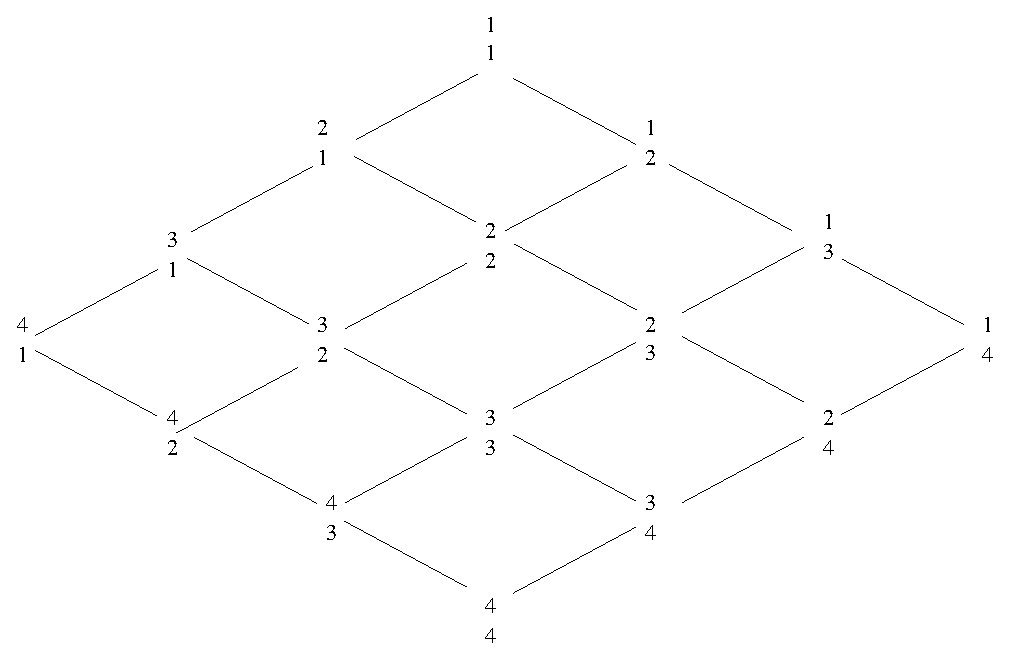
\includegraphics{figures/latt1.eps}}}
\caption{\label{latt:1}Lattice of NDs for a relation of 2 FDs
(not shown) and maximum domain size of 4 for each dependency}
\end{figure}

\index{Numerical Dependency!Maximal Set}
\begin{definition}[Maximal set of NDs]
\begin{rm}
The {\em maximal} set of NDs of $r$ with respect to F,
denoted by $maximal(r$, F), is the maximal set N of NDs
in ${\cal L}_m$(F) (with respect to $\sqsubseteq$) such that $r
\models$ N.$\quad\Box$ 
\end{rm}
\end{definition}
\medskip

Given $r$ and F, $maximal(r$, F) can be computed in polynomial time in the
sizes of $r$ and F by a straightforward hill climbing procedure
on ${\cal L}_m$(F), illustrated in algorithm~\ref{alg:mu}. For each X $\to$ A $\in$ F this procedure finds 
the minimal $k$ such that $r \models$ X $\to^k$ A, starting 
from X $\to^m$ A which $r$ trivially satisfies since $\mid r \mid = m$. 

\index{Numerical Dependencies!improvement set}
\begin{definition}[Improvement set of a set of NDs]
\begin{rm}
The {\em improvement set} of $r$ with respect to F, 
denoted by $\mu$($r$, F), is defined as 
\begin{displaymath}
\mu(r, {\rm F}) = \{{\rm X} \to^k {\rm A} \mid 
{\rm X} \to^k {\rm A} \in maximal(r, {\rm F}) \mbox{ and }  k > 1\}.
\end{displaymath}
Algorithm~\ref{alg:mu} returns the {\em improvement set} of $r$ if any FDs
satisfied in $r$ are removed from N.$\quad\Box$
\end{rm}
\end{definition}
\medskip


{\renewcommand{\baselinestretch}{1}
\begin{figure}[ht]
\begin{center}
\fbox{\begin{minipage}{14cm}
\begin{algorithm}[{\rm MU}($r$, {\rm F})]\label{alg:mu}
\begin{rm}
\begin{tabbing}
t1\=t2\=t3\=t4\=t5\= \kill \\
1.  \> \> {\bf begin} \\
2.  \> \> \> $m$ := $\mid r \mid$; \\
3.  \> \> \> N := the bottom element of $\mathcal{L}_m$ (F); \\
4.  \> \> \> {\bf while} $\exists$ G such that N $\cover$ G {and} $r \models$ G  {\bf do} \\
5.  \> \> \> \> N := G; \\
6.  \> \> \>  {\bf end while} \\
7. \> \> \> {\bf return} N;  \\
8. \> \> {\bf end.}
\end{tabbing}
\end{rm}
\end{algorithm}
\end{minipage}}
\end{center}
\caption{\label{numdep:fig:mu} The improvement algorithm for NDs}
\end{figure}
}

\subsection{Similarity Measures and Numerical Dependencies}
\index{Similarity Measure!ND}

We introduce a measure for calculating the proximity of two ND sets using
their position within the lattice.  We show that this measure is a distance
function, satisfying reflexivity and symmetry, and is also a metric, 
satisfying the triangle inequality. Firstly, we begin by defining the best
approximation given by a set of NDs to their functional counterparts.
We define the {\em size} of a set of NDs N to be the number of attributes 
appearing in N including repetitions and define a {\em step}, either up
or down, to be exactly minus or plus one, respectively, to a single branch of
one ND within an ND set. 

\begin{definition}[The best approximation of a set of FDs]\label{def:best}
\begin{rm}
A set of NDs N over R is the {\em best approximation} of 
a set of FDs F over R with respect to a relation $r$ over R,
with $\mid r \mid = m+1$ (or simply the best approximation of F
if $r$ is understood from context), if $r \models$ N 
and there does not exist a set of NDs, $N^\prime \in {\cal L}_m$
such that N $\cover$ $N^\prime$ and $r \models N^\prime$.$\quad\Box$
\end{rm}
\end{definition}



\begin{proposition}[The number of NDs higher in the Lattice]
\begin{rm}
Given an ND set $N$ = \linebreak[4]   $\{ X_1 \to^{k_1} A_1, X_2 \to^{k_2} A_2,
 \ldots, X_n \to^{k_n} A_n \}$, the number of ND sets above this set in the
lattice is ($k_1 \cdot k_2 \cdot \ldots \cdot k_n$) - 1.
\end{rm}
\end{proposition}

{\em Proof.} An ND is higher in the lattice if within a 
set of NDs none of the $k_i$ branches have any values higher than
any of those in the set {\em and} at least one of the NDs has some 
$k_j$ branch value
lower than one of those in the set. Each ND $X_i \to^{k_i} A_i$ within
the set can take $k_i$ values. We consider all permutations of these
values to get $k_1 \cdot k_2 \cdot \ldots \cdot k_n$ from which we 
must ensure that the ND set values of $N$ itself is not included to get
$k_1 \cdot k_2 \cdot \ldots \cdot k_n$ - 1. $\Box$

\smallskip

This provides us with the basis for a distance measure between an ND set
and its functional representation. However,  using this technique allows,
in some instances, ND sets which are the same number of steps below the
FD equivalent to have different values. This is due to ND sets containing
FDs or NDs which are close to being functional having less sets above them
in the lattice. To illustrate, if we have two ND sets $N_1,N_2$ each containing two NDs such that $N_1$ has dependencies with 4 and 2 as branches whilst $N_2$ has dependencies with 3 and 3 as branches then $N_1$ will have fewer ND sets
above it in the lattice though both are the same number of steps from their
functional equivalent, shown in Figure~\ref{latt:1}. We now introduce the 
metric we used in our simulations
and note that if we are interested in comparing ND sets with either more 
or less {\em near} FDs we can refer to the above measure 
whenever the metric provides the same distance.
\smallskip

In the following definition {\em distance} is defined as the number of
{\em steps} in the lattice. In Definition~\ref{def:nd_prox} we
use proposition~\ref{prop:maxdist} to prove that the denominator for
this measure is normalised for any two NDs within a given
relation. $p(N_1,N_2)$ provides a suitable measure of proximity
between two ND sets. We use the measure of
Definition~\ref{def:nd_prox} in our simulations presented in
Chapter~\ref{chap:consistency} in the following form: Given a set of NDs $N_1$ and a set of FDs $F$, which $N_1$ approximates,
then the proximity between the two dependency sets is given by
$p(N_1,F)$. 
\index{Numerical Dependency!Proximity measure}
\begin{definition}[Proximity between two ND sets]\label{def:nd_prox}
\begin{rm}
Given two sets of NDs $N_1$ and $N_2$ we define the metric as follows: 
\[
p(N_1,N_2) = \frac{\Sigma_{i = 1, 2} \mbox{ Distance from } N_i \mbox{ to }  lub \{ N_1, N_2 \}}
{\mbox{Maximum distance between any two ND sets to their $lub$ in the lattice}}
\quad\Box\]
\end{rm}
\end{definition}

We define the bottom of the
lattice to be the set of NDs with each branching factor equivalent to
the domain size of the attribute on the right hand side of each
ND, assuming a finite domain size.

\smallskip
\begin{proposition}\label{prop:maxdist}
\begin{rm}
The maximum distance between any two points in
the lattice to their $lub$ is always equivalent to the
distance from the bottom to the top of the lattice. 
\end{rm}
\end{proposition}

{\em Proof}. We prove this by induction on the NDs within the two ND sets.\newline 
\smallskip
\indent ({\em Basis}): We see that if $N_1$ and $N_2$ are empty then the
result is immediate.

\smallskip

({\em Induction}): We have two ND sets $N_1$ and $N_2$ which are distance
$d$ apart where $d \le q$ and $q$ is the maximum distance apart between
any two ND sets. We add an ND $X \to^{k_1} Y$
to $N_1$ and $X \to^{k_2} Y$ to $N_2$ which differ only
on their branching factor. Without loss of generality, if $k_1 < k_2$ then the
distance apart between $N_1$ and $N_2$ becomes $d + k_2 - k_1$. This 
remains less than or equal to the maximum distance apart which is $q + k'_2 -
k'_1$ where, without loss of generality, $k'_1 = 1$ (it is an FD) and
$k'_2$ is at the bottom of the lattice. $\Box$

\smallskip

The measure $p$ is a distance function given that the distance
between two NDs is zero only when they are equivalent and that 
$p(n_1,n_2) = p(n_2,n_1)$ always holds. It also satisfies the 
triangle inequality, whose proof we now outline. This implies
therefore that $p$ is a metric implying that sets with a common value
can be compared.

\begin{theorem}
\begin{rm}
Given three ND sets, $N_1$, $N_2$, and $N_3$, $p(N_1,N_2) + p(N_2,N_3)
\ge p(N_1,N_3)$.
\end{rm}
\end{theorem}
\smallskip

{\em Proof.} We show that if $N_1$, $N_2$ and $N_3$ are non-empty and the 
triangle
inequality holds then the addition of a new ND to each set which may
differ only on its branching factor will still satisfy the triangle inequality.
Assume we add three NDs $X \to^{k_i} A$ with $i = 1,2,3$ to $N_1,N_2$ and
$N_3$, respectively. We also assume, without loss of generality, that 
$k_1 < k_3$. We denote each ND set $N_i \cup \{ X \to^{k_i} A \}$ by $N'_i$
for $i = 1,2,3$. We perform induction on the NDs in each set.

\smallskip
({\em Basis}): If $N_1$ = $N_2$ = $N_3$ = $\emptyset$ then the 
result is immediate.

\smallskip
({\em Induction}):
 We assume that $k_2 \le k_1$, then $p(N'_1,N'_2)$ =
distance from $N_1$ to $lub(N_1,N_2)$ + distance from $N_2$ to $lub(N_1,N_2)$ +
$k_2 - k_1$. Similarly for $p(N'_2,N'_3)$ and $p(N'_1,N'_3)$ we have the
additional components, $k_3 - k_2$ and $k_3 - k_1$. Therefore, we have
$p(N'_1,N'_2) + p(N'_2,N'_3)$ = $p(N_1,N_2) + k_1 - k_2 + p(N_2,N_3) +
k_3 - k_2$ and $p(N'_1,N'_3)$ = $p(N_1,N_3) + k_3 - k_1$. We know that  
$p(N_1,N_2) + p(N_2,N_3) \ge p(N_1,N_3)$ holds and we see
 that  $k_1 - k_2 + k_3 - k_2 \ge k_3 - k_1$ holds if $k_1 \ge k_2$ which
is true, based on our initial assumption. We can similarly prove the 
triangle inequality for the case when $k_1 \le k_2$. $\Box$


\subsection{Partitioning a Relation for Mean NDs}\label{nd:subsec:mean}
\index{Numerical Dependency!Mean ND}
In many data mining tools it is important that there exist measures
which accurately reflect the content of the database; this motivates
us to define mean ND set satisfaction for some situations like that of
Example~\ref{ex:mean_nd}.

\smallskip

In Chapter~\ref{chap:review} we presented Definition~\ref{def:nd_part}
for partitioning of a relation into blocks for an ND X $\to^k$ Y which
agree on X.
The satisfaction of an ND X $\to^k$ Y implies only that there exists
at least one partition ${\cal B}$ which contains at least $k$ tuples
with at most $k$ different Y-values.  There may however be numerous
other partitions on X which may have far less than $k$ different
Y-values and so the partition ${\cal B}$ dominates the relation and
presents an inaccurate representation of the proximity to FD set
satisfaction.  We therefore define the {\em mean numerical dependency}.

\index{Numerical Dependency!Mean ND}
\index{Mean ND}
\begin{definition}[Mean Numerical dependency]\label{def:mean_nd}
\begin{rm}
A {\em mean numerical dependency} over R (or simply a mean ND)
is a statement of the form X $\to^{\bar{k}}$ Y, where X, Y $\subseteq$ R and
$\bar{k} \ge 1$. We refer to $\bar{k}$ as the {\em mean branching
factor}.$\quad\Box$ 
\end{rm}
\end{definition}
\index{Mean ND!Satisfaction}
\begin{definition}[Satisfaction of a Mean ND]\label{def:sat-mean_nd}
\begin{rm}
Let $r$ be a relation over R.
An ND X $\to^{\bar{k}}$ Y is {\em satisfied} in $r$,
denoted by $r \models$ X $\to^{\bar{k}}$ Y, such that $r$ is
partitioned into blocks 
$\{{\cal B}_1, {\cal B}_2, \ldots, {\cal B}_w\}$ with respect to X
$\to$ Y such that $\bar{k} = \frac{\sum_{i = 1}^{w} \mid
\pi_{\rm Y}({\cal B}_{i}) \mid }{w}$.
A set of averaged NDs $\bar{\rm N}$ is {\em satisfied} in $r$,
denoted by $r \models$ $\bar{\rm N}$, whenever
$\forall$ X $\to^{\bar{k}}$ Y $\in$ $\bar{\rm N}$, $r \models$ X
$\to^{\bar{k}}$ Y.$\quad\Box$ 
\end{rm}
\end{definition}



\begin{example}\label{ex:mean_nd}
\begin{rm}
We assume that a relation $r$ over AB satisfies the ND A $\to^{14}$ B
as its closest approximation to the FD A $\to$ B. However $r$ may, for
example, only
contain three partitions $\{{\cal B}_1, {\cal B}_2, {\cal B}_3\}$
with each partition satisfying the NDs A $\to^{14}$ B, A $\to^{1}$ B,
and A $\to^{1}$ B, respectively. We note the last two are satisfied
functionally. The mean ND set satisfaction is A $\to^{\bar{5.67}}$ B.
Within a block $\cal B$ the number of tuples is not related to
the branching factor value, given by $\mid \pi_{\rm B}({\cal B}) \mid$.
\end{rm}
\end{example}

In our work on indefinite information in relations we remark that we
are interested in exact ND set satisfaction only, given the nature of
the problem. In the data mining of NDs in standard and temporal
relations we may often be interested in the mean ND set satisfaction
value. We note that if this value is vastly different from the exact
satisfaction value then it is likely that one or more partitions from
the relation {\em dominate} and remaining partitions will satisfy the
NDs more functionally.

\section{The Chase Procedure for NDs}\label{sec:nd_chase}
\index{Chase Procedure!for NDs}

We now show how CHASE($r$, F) can be generalised to CHASE($r$, N), where N is
a set of NDs over R, shown in Figure~\ref{numdep:fig:nd_chase}.

{\renewcommand{\baselinestretch}{1}
\begin{figure}[ht]
\begin{center}
\fbox{\begin{minipage}{16cm}
\begin{algorithm}[{\rm CHASE}($r$, {\rm N})]\label{alg:ndchase}
\begin{rm}
\begin{tabbing}
t1\=t2\=t3\=t4\=t5\=t6\=t7\= \kill \\
\ra.  \> \> {\bf begin} \\
\sa.  \> \> \> Result := $r$; \\
\sa.  \> \> \> Tmp := $\emptyset$; \\
\sa.  \> \> \> {\bf while} Tmp $\not=$ Result {\bf do} \\
\sa.  \> \> \> \> Tmp := Result; \\
\sa.  \> \> \> \> {\bf if} $\exists$ X $\to^k$ Y $\in$ N, $\exists t_1, t_2, \ldots, t_k, t_{k+1} \in$ Result such that  \\
    \> \> \> \> \> $t_1$[X] = $t_2$[X] = $\ldots$ = $t_k$[X] = $t_{k+1}$[X] \\
    \> \> \> \> \> but $t_1$[Y] $\not=$ $t_2$[Y] $\not= \ldots \not=$ $t_k$[Y] $\not=$ $t_{k+1}$[Y] {\bf then} \\ 
\sa. \> \> \> \> \> {\bf for each} $A \in$ Y$-$X {\bf do} \\
\sa. \> \> \> \> \> \> \> $t_i$[A],$t_j$[A] := max($t_i$[A],$t_j$[A])
    for two distinct values $i,j \in 1,\ldots,k+1$; \\
\sa. \> \> \> \> \> {\bf end for} \\
\sa.  \> \> \> \> {\bf end if} \\
\sa.  \> \> \> {\bf end while} \\
\sa. \> \> \> {\bf return} Result;  \\
\sa. \> \> {\bf end.}
\end{tabbing}
\end{rm}
\end{algorithm}
\end{minipage}}
\end{center}
\caption{\label{numdep:fig:nd_chase} The Chase procedure for NDs}
\end{figure}
}

We leave it to the reader to verify that when $k = 1$, i.e. X $\to^k$ Y is an
FD, then CHASE($r$, N) reduces to CHASE($r$, F).


\begin{lemma}\label{th:algterm}
\begin{rm}
Algorithm~\ref{alg:ndchase} terminates.
\end{rm}
\end{lemma}

{\em Proof.} No new values are introduced into the algorithm at any
step and therefore the algorithm must halt after executing the while
loop a finite number of times. $\Box$

\begin{theorem}\label{th:chase}
\begin{rm}
Given a set of NDs, N, then $\forall n \in N$, CHASE($r$, N) $\models n$.
\end{rm}
\end{theorem}

{\em Proof.} Direct from the definitions of the algorithm and of ND
satisfaction. $\Box$

We also note in theorem~\ref{th:chase} that if $r \models$ N, for a
relation $r$ and an ND set N then \linebreak CHASE($r$, N) = $r$.
We return to the chase procedure and show how it can be used as an
inference procedure in Section~\ref{subsec:nd_ch_inf}, after discussion of the
axiomatisation of NDs.   

\section{Inferences for Numerical Dependencies}\label{sec:nd_inf}

The axiom system given in \cite{gm85a} is shown to be sound and
complete only in the special cases of, for a schema R, either $|$R$| \le 3$ or when the number of
NDs with $k > 1$ is at most one. \cite{gm85b} extends this result
and shows that there is no finite sound and complete
axiomatisation for NDs. 

\subsection{ND Axiomatisation}\label{subsec:nd_axiom}
\index{Numerical Dependency!Axiomatisation}
\index{Numerical Dependencies!Inference Rules}
NDs allow a more general dependency relation than functional
dependencies.  \cite{gm85a,gm85b} introduce NDs with regard
to obtaining normal forms which avoid or minimise redundancy, from a
database with $k$-dependency constraints. Grant and Minker also
provide an axiomatisation for NDs which is a
generalisation of the Armstrong axioms for 
FDs. \cite{gm85a} presents a set of sound
inference rules for NDs. \cite{gm85b} 
shows that there does not exist a {\em finite} set of sound and
complete inference rules for Numerical Dependencies.
These axioms are shown to be complete for relations which have, at most,
3 attributes.  It is shown that any relation with more than 3 attributes is
not complete. We show in Section~\ref{subsec:nd_ch_inf} how the chase may
be used as an inference procedure.
If the relation utilises only FDs then the axioms
contain the Armstrong rules as a subset.\\

For clarity, we now present inference rules 1-5 from \cite{gm85b}:
\begin{description}
\item[R1] If Y $\subseteq$ X then infer X $\to$ Y
\item[R2] From X $\to^k$ Y infer ZX $\to^k$ ZY
\item[R3(a)] From X $\to^k$ Y and Y $\to^j$ Z infer X $\to^{k \cdot j}$ YZ
\item[R3(b)] From X $\to^k$ Y and Y $\to^j$ Z infer X $\to^{k \cdot j}$ Z
\item[R4] From X $\to^k$ Y infer X $\to^{k + 1}$ Y
\item[R5$_m$] From  $\{ X \to^{2} Y_i \quad |  \quad 1 \le i \le 3m-2
\}$  \\
$\quad \cup$ $\quad \{ Y_{i1}Y_{i2} \ldots Y_{im} \to Z
\quad |  \quad 1 \le i1 < i2 < \ldots < im \le 3m-2 \}$ infer $X \to^{2} Z$
\end{description}

Rules R1,R2 and R3(b) are extensions of the axioms for FDs.
We now present another inference rule which generalises the rule
R5$_m$ of \cite{gm85b}, R6$_{k,m}$, which can be viewed as a generalised
transitivity rule for NDs wherein a bound on the number of attributes
required for inference is created based on the branching factor of the
NDs {\em and} the number of attributes on the left hand side of the FD
which determines attribute $Z$. R6$_{k,m}$ is a useful extension to
the class of transitive axioms for NDs.

\smallskip
{\line
\begin{table}[ht]
\begin{tabular}{cl} \\
(R6$_{k,m}$): 	& From  $\{ X \to^{k} Y_i \quad |  \quad 1 \le i \le
		\eta \}$    $\quad \cup$ \\
		&    $\quad \{ Y_{i1}Y_{i2} \ldots Y_{im} \to Z
		\quad |  \quad 1 \le i1 < i2 < \ldots < im \le \eta \}$ \\ 
\rule{0cm}{5mm} & we can infer $X \to^{k} Z$ where $\eta =
		(m-1){k+1 \choose 2} + 1$  \\
\end{tabular}
\end{table}}
\smallskip

\begin{theorem}\label{th:1}
\begin{rm}
Each rule R6$_{k,m}$ is sound and has minimal hypothesis.
\end{rm}
\end{theorem}

{\line
\begin{table}[ht]
\begin{center}
\begin{tabular}{|c|c|c|c|c|c|} \hline
X	&	Y$_i$	&	Y$_2$	& $\ldots$ & Y$_{\eta}$	 & Z \\\hline
1	&		&		&          &	       & 1 \\
1	&		&		&          &	       & 2 \\	
$\vdots$ &		&		&          &	       & $\vdots$ \\
1	&		&		&          &	       & $k+1$\\ \hline
\end{tabular}
\end{center}
\caption{\label{tbl:axiom_r6km} Example relation for proof of axiom R6$_{k,m}$}
\end{table}}	


{\em Proof.} We assume that we have a relation $r$ with $\eta + 2$
attributes and $k+1$ cells, as in Table~\ref{tbl:axiom_r6km}, and that
X agrees on all of its $k+1$ cells.  We also assume, from 
R6$_{k,m}$, that X $\to^k$ Y$_i$ holds for all $1 \le i \le \eta$ and
that for a given $m$ all possible FDs of the form \linebreak Y$_{i1}$Y$_{i2}$ $\ldots$
Y$_{im}$ $\to$ Z hold for 1 $\le i1 < i2 < \ldots < im \le \eta$ and
that X $\to^k$ Z does not hold.
Each X $\to^k$ Y$_i$ implies that each Y$_i$ attribute must agree on
at least two cells. In a relation with $k + 1$ tuples there are 
${k+1 \choose 2}$ ways in which a single
attribute may agree on two tuples. For some set of attributes
Y$_{i1}$Y$_{i2}$ $\ldots$ Y$_{im}$ 
in Y$_1$ to Y$_{\eta}$ if $\eta = (m-1){k+1 \choose 2} + 1$, then at
least one FD of the form \linebreak Y$_{i1}$Y$_{i2}$ $\ldots$
Y$_{im}$ $\to$ Z must agree on all of its Y$_i$ attributes. This is due to
exhaustion of all possible combinations on which two tuples may agree.
Whichever tuples agree on all $m$ attributes imply that Z also agrees
on these attributes. Therefore there may not be $k+1$
different values on Z and we have a contradiction. 
\medskip

We prove the minimal hypothesis by noting that if any FD X $\to^k$ Y
or \linebreak Y$_{i1}$Y$_{i2}$ $\ldots$
Y$_{im}$ $\to$ Z for 1 $\le i1 < i2 < \ldots < im \le \eta$ is
omitted from our requirements then there exists a counterexample which
does not imply X $\to^k$ Z for some combination of values on the
attributes in Y$_1$ to Y$_{\eta}$. $\Box$

\smallskip

We can also prove this as for R5$_m$ in \cite{gm85b} by explicitly
proving that no counterexample relation exists.
We note that when $k$ = 1 then R6$_{k,m}$ reduces to transitivity of FDs,
and when $k$ = 2 then $\eta = 3m - 2$, the figure given in
\cite{gm85b} for R5$_m$. 


\subsection{The Chase as an Inference Procedure}\label{subsec:nd_ch_inf}
\index{Chase Procedure!for ND inference}

We prove that the chase is a 
sound and complete inference procedure for NDs. In the sequel, we
assume that NDs have singleton right hand sides.

Given a set of NDs $N$ and an ND $\sigma$, we apply the chase as an
inference tool to discover if $N \models \sigma$. 
We create a relation $r_\sigma$ which for $\sigma = X \to^k
A$ has $k+1$ tuples with $k+1$ different values on attribute set $A$,
all values on X equivalent and all values in $R \backslash XA$ unique.
We need to consider all possible iterations of the chase procedure,
presented in algorithm~\ref{alg:ndchase}, for a relation $r_\sigma$
for the inference procedure to be sound and complete, given that one
instance of the chase may not terminate with a unique end result,
known as the {\em Church-Rosser} property \cite{mms79}. We refer to
each complete application of the chase as a {\em chase sequence}.

{\line
\begin{table}[ht]
\begin{center}
\begin{tabular}{c|c|c|c|c|c|c|c|} \cline{2-8}
 		& X$_1$ 	& $\ldots$ 	& X$_m$ & A 	& B$_1$ & $\ldots$ 	& B$_m$ \\ \cline{2-8}
$t_1$ 		& 1  		& $\ldots$ 	& 1	&  1  	& 1 	& $\ldots$ 	& 1 \\
$t_2$ 		& 1  	& $\ldots$ 	& 1&  2  	& 2 	&  $\ldots$ 	& 2 \\
$\vdots$ 	& $\vdots$  &  $\ddots$ & $\vdots$  &  $\vdots$  & $\vdots$ & $\ddots$ & $\vdots$ \\
$t_{k+1}$ 	& 1  &  $\ldots$  &  1  & $k+1$  & $k+1$ & $\ldots$ 	& $k+1$ \\ \cline{2-8}
\end{tabular}
\end{center}
\caption{\label{tbl:rel_chase1} Relation to be chased by ND set N with
$\sigma = X \to^k A$, X = $\{ X_1, \ldots, X_m \}$, R $\backslash$ XA = $\{ B_1, \ldots, B_m \}$
and $m$ = $|$ R $\backslash$ XA $|$}
\end{table}}	


We motivate theorem~\ref{th:3} by showing an example relation where
different sequences of tuples modified by the chase produce different
results. We show this for an ND set \linebreak N = $\{$ X $\to^2$ 
B$_1$,  X $\to^2$ B$_2$, B$_1$B$_2$ $\to$ A $\}$, $\sigma$ = X $\to^2$
A, and relation $r_1$ in
Table~\ref{tbl:NDchase1}. 
 For two different chase sequences, with different tuples modified, we have
$r_{1}^c$ 
$\not\models$ X $\to^2$ A, shown in Table~\ref{tbl:NDchase2}, and $r_{1}^c$ 
$\models$ X $\to^2$ A, shown in Table~\ref{tbl:NDchase4}.
Therefore 
N $\not\models$  X $\to^2$ A, which may not have been discovered if
we had only examined one chase sequence.

{\line
\begin{table}[ht]
\begin{center}
\begin{tabular}{|c|c|c|c|} \hline
 {\bf X} & {\bf B$_1$} & {\bf B$_2$} & {\bf A} \\\hline
 1 & 1 & 1 & 1 \\ 
 1 & 2 & 2 & 2 \\ 
 1 & 3 & 3 & 3 \\ \hline
\end{tabular}
\end{center}
\caption{\label{tbl:NDchase1}$r_1$ before CHASE procedure} 
\end{table}
}

{\line
\begin{table}[ht]
\begin{minipage}[b]{7cm}
\begin{center}
\begin{tabular}{|c|c|c|c|} \hline
 {\bf X} & {\bf B$_1$} & {\bf B$_2$} & {\bf A} \\\hline
 1 & 1 & 2 & 1 \\ 
 1 & 3 & 2 & 2 \\ 
 1 & 3 & 3 & 3 \\ \hline
\end{tabular}
\end{center}
\caption{\label{tbl:NDchase2}Example CHASE($r_1$,N) after CHASE procedure} 
\end{minipage}
\hfill
\begin{minipage}[b]{7cm}
\begin{center}
\begin{tabular}{|c|c|c|c|} \hline
 {\bf X} & {\bf B$_1$} & {\bf B$_2$} & {\bf A} \\\hline
 1 & 1 & 1 & 1 \\ 
 1 & 3 & 3 & 3 \\ 
 1 & 3 & 3 & 3 \\ \hline
\end{tabular}
\end{center}
\caption{\label{tbl:NDchase4}Counterexample CHASE($r_2$,N) after CHASE procedure } 
\end{minipage}
\end{table}
}


Theorem~\ref{th:2} requires the notion of containment mapping
cf. \cite{atze93}.  We define a function $dom$ which
returns the active domain of a relation.

\begin{definition}[Containment Mapping]\label{def:cm}
\begin{rm}
A containment mapping $\phi$ from $r_\sigma$ to a relation $r$ has
each value in $dom$($r_\sigma$) mapped by $\phi$ to a value in $dom$($r$).
This is extended to tuples over $R = A_1A_2 \ldots A_m$ as $\phi(t) =
\phi(t[A_1]),\phi(t[A_2]),\ldots, \phi(t[A_m])$ and extends to a
relation as $\phi(r) = \{ \phi(t) | t \in r \}$.$\quad\Box$ 
\end{rm}
\end{definition}


\begin{theorem}\label{th:2}
\begin{rm}
Given a set of Numerical Dependencies N and a ND $\sigma = X \to^k A$,
N $\models \sigma$ iff $\neg\exists t^c_1[A] \not= t^c_2[A] \not= \ldots
\not= t^c_{k+1}[A]$ where $t^c_1,t^c_2,\ldots,t^c_{k+1} \in
r_\sigma^c$ and $r_\sigma^c$ = chase($r_\sigma$,N) for all possible
sequences of the chase.
\end{rm}
\end{theorem}

\index{Soundness!of the chase for NDs}
\index{Completeness!of the chase for NDs}

{\em Proof. (if)} We assume that $A \not\subseteq X$. We let $r$ be a
relation over $R$ such that $r \models N$; we show that $r \models
\sigma$. Let $t_1, t_2, \ldots, t_{k+1} \in r$ such that $t_1[X] =
t_2[X] = \ldots = t_{k+1}[X]$. We claim that for some $i,
j \in \{1, 2, \ldots, {k+1}\}$ there exists $t_i[A] = t_j[A]$. 

\smallskip
Let $\phi$ be a containment mapping from $r_\sigma$
$\phi(u_1) = t_1$, $\phi(u_2) = t_2$, $\ldots$, $\phi(u_{k+1}) = t_{k+1}$. We
shall prove that $\phi$ is additionally a containment mapping from
CHASE($r_{\sigma}$, N) to $r$ so that for some $i,j \in r_{\sigma}^c$,
$\phi(t_i^c[A])$ = $\phi(t_j^c[A])$ implies $t_i[A] = t_j[A]$. This is
the case for all possible chase sequences on $r_\sigma$. 

\smallskip
We prove this by induction on the number of steps, $s$, required to compute
CHASE($r_{\sigma}$, N).

\smallskip

({\em Basis}):
If $s = 1$ then for some ND $W \to^k B \in N$ two values are equated 
in $B$ where \linebreak $W \subseteq X$ and $A = B$ so therefore $u_i[A] =
u_j[A]$ implying that $\phi(u_i[A]) = t_i[A]$ and \linebreak $\phi(u_j[A]) =
t_j[A]$ and so $t_i[A] = t_j[A]$ for some $i,j$ in $r$.
\smallskip
 
({\em Induction}):
We assume that the result holds when $s$ steps of the chase procedure
are required. We now prove it to be true when $s+1$ chase steps are
required. We let the $s+1$ chase step be for an ND $W \to^k B$ and
$u_i, u_j$ be two tuples in $r_\sigma$ such that the $s+1$ step either modifies
$u_i$ or $u_j$. Thus, for $B$ either $u_i[B]$ or 
$u_j[B]$ is modified so that $u_i[B] = u_j[B] = t_i^c[A] = t_j^c[A]$.
Now, given $u_i[W] = u_j[W]$ then $\phi(u_i[W]) = \phi(u_j[W])$ by the
definition of containment mapping.  Therefore $\phi(t_i^c[A]) =
\phi(t_j^c[A]) = \phi(u_i[B]) = \phi(u_j[B]) = t_i[A] = t_j[A]$ holds, since $r_{\sigma}
\models W \to^k B$. Given that $\phi$ only differs from the result of
$s$ steps on $u_i[B]$ or $u_j[B]$ it is a containment mapping from
$r_\sigma^c$ in all possible chase sequences. In any sequence, if
$t_i^c[A] = t_j^c[A]$ we have, by definition of $\phi$, $t_i[A] = t_j[A]$.

\smallskip

{ \em (only-if)} If, in some chase sequence, there does not exist
$t_i^c[A] = t_j^c[A]$ for 
some $i,j \in {1,2, \ldots, k+1}$ then we can
construct a relation $r$ 
which satisfies all $n \in N$ but violates $\sigma$.  
\smallskip
Alternatively, the chase for $r_\sigma$ can be shown to be isomorphic
to a relation $r$ which satisfies N but violates X $\to^k$ A by
mapping each value in $r_{\sigma}^c$ to a value in $dom(r)$. $\Box$



\begin{corollary}\label{th:3}
\begin{rm}
The chase inference procedure for Numerical Dependencies is sound and
complete.
\end{rm}
\end{corollary}

{\em Proof.} Soundness and completeness of the chase as an inference
procedure is a corollary of theorem~\ref{th:3}. $\Box$

\smallskip
The existence of a sound and complete chase procedure shows that
implication on NDs is decidable. The implication
problem for NDs is in co-NP, used to denote that the complementary
no/yes problem is in the 
set NP \cite{gj79}; we know that the converse
problem is NP given that we can {\em guess} a relation  (equivalent to
a complete sequence of the chase procedure) 
$r_\sigma^c$ 
and verify in polynomial time whether or not
$r_\sigma^c$ $\models$ $\sigma$. NP-completeness remains an open problem.


\subsection{Armstrong Relations for NDs}\label{subsec:nd_ar}
\index{NDs!Armstrong Relations for}

Within a finite relation there does not exist an
Armstrong Relation, defined for FDs in Definition~\ref{def:AR}, for a
set of NDs N, unless N contains all possible 
combinations of attribute sets. We may prove this as follows. Assume that we
are given a set of NDs N and that $\sigma$ is an ND X $\to^k$ Y such that
N $\not\models \sigma$. For any relation $r$ such that $r \models$ N we
have, at least, $r \models \sigma$ where $k = \mid r \mid$.

\medskip
We therefore define a weak AR for an ND set N.
\index{Armstrong Relations!for NDs}

\begin{definition}[A Weak Armstrong Relation]\label{def:weak_AR}
\begin{rm}
A relation $r$ is a weak AR for a set of NDs N if $r \models$ N and
$\forall \sigma$ such that N $\not\models \sigma$ then $r \models
\sigma$ maximally 
with respect to $k_\sigma$ implying that $r$ satisfies all NDs
$\sigma$ with a branching 
factor no higher than $k_\sigma$. The choice of a value for $k_\sigma$
may be related to branching factors of NDs in N (or the size of the
relation).$\quad\Box$ 
\end{rm}
\end{definition}

These weak Armstrong Relations would extend the practical application
of NDs within database design tools by helping designers think of what
NDs may be required via examination of an actual relation. 

\section{Numerical Dependencies in Data Mining}\label{sec:nd_datamine}
\index{Numerical Dependency!in data mining}
We now briefly present data mining for numerical dependencies in
standard relations. We emphasise the following:
\begin{itemize}
\item In contrast with functional dependency approximation data mining
we are not seeking to assess what proportion of a relation satisfies a
functional relationship, cf. Table~\ref{tbl:fd_approx} and
\cite{hkp98,km95}. We seek to discover 
generalisations of FDs when the FD may be viewed as too strict.
\item In our work on temporal and indefinite relations we assume the
user provides a ND set upon which we seek instances of ND
satisfaction. The use of NDs in a blind discovery context would
generate ND satisfying instances for all possible attribute set
combinations, which is not practical due to the complexity.
\end{itemize}

\subsection{Dependency Mining Applications}\label{subsec:fd_jobs}
\index{Dependency Data Mining!using NDs}
Approximation of the dependency set, possibly approximated using numerical
dependencies, on a large database in existence may reveal unknown information
in the form of these dependencies which may hold in the database. A
recent work on the reverse-engineering, or discovery if you will, of
cardinality constraints for inference of the ER-model is presented in
\cite{sou98}. From lemma~\ref{rev:lem_cc} this is another application
for ND discovery.

\smallskip

Applications for dependency mining include a database
design tool which the database designer can use in conjunction with a possible
instance of the data to be stored within the database.  Inference upon this 
example set will then provide the designer with vital information as to possible
unknown dependencies that be satisfied in the relation. The approach of 
Bell and Brockhausen \cite{bb95} in making inferences from the verified and
invalid data dependencies is aimed at {\em supporting} the database
designer. Example~\ref{nd:ex_nd_app} shows an application of ND discovery.


\begin{example}\label{nd:ex_nd_app}
\begin{rm}
In a patient database within a hospital every patient visit is
independently stored within a {\em patient} details relation and a {\em
disease/symptom/treatment} relation.  
Given a numerical dependency specified $DISEASE \to^{10} SYMPTOM$ stating
that a disease can have at most 10 symptoms, it may however be approximated
that $ADDRESS \: \: \: PATIENT \to^{6} SYMPTOM$ showing that at most
6 of the symptoms can occur at the same location for a patient.
\end{rm}
\end{example}


\subsection{Mining a relation for a set of NDs}

We consider only singleton right hand sides. For a relation $r$ over R with
$n$ attributes we have $n 2^{n-1}$ NDs returned by this algorithm and
so in Figure~\ref{graph:nd_mine1} we only give results obtained from
restricting the 
left hand sides to a given arity of 
attributes. Algorithm~\ref{alg:mine} uses Algorithm~\ref{alg:mu} to
generate the ND satisfied from an FD template.

\medskip

{\renewcommand{\baselinestretch}{1}
\begin{figure}[ht]
\begin{center}
\fbox{
\begin{minipage}{16cm}
\begin{algorithm}[{\rm ND\_mine}($r$, {\rm R})]\label{alg:mine}
\begin{rm}
\begin{tabbing}
t1\=t2\=t3\=t4\=t5\=t6\=t7\=t8\=t9\= \kill \\
\ra.  \> \> {\bf begin} \\
\sa.  \> \> \> ND\_set := $\emptyset$;\\
\sa.  \> \> \> {\bf for each} A $\in$ R {\bf do}\\
\sa.  \> \> \> \> {\bf for each} W $\in \mathcal{P}$(R - A) {\bf do}\\
\sa.  \> \> \> \> \> $\{$ W $\to^k$ A $\}$ =  MU($r$, $\{$ W $\to$ A $\}$); \\
\sa.  \> \> \> \> \> ND\_set := ND\_set $\cup$ $\{$ W $\to^{k}$ A $\}$; \\
\sa. \> \> \>  \> {\bf end for}; \\
\sa. \> \> \>    {\bf end for}; \\
\sa. \> \> \> {\bf return} ND\_set;  \\
\sa. \> \> {\bf end.}
\end{tabbing}
\end{rm}
\end{algorithm}
\end{minipage}}
\end{center}
\caption{\label{numdep:fig:nd_mine} The ND mining algorithm}
\end{figure}
}

The computational complexity of algorithm~\ref{alg:mine} is O($n^2 2^{n-1}
\mid r \mid log \mid r \mid$). There are $n2^{n-1}$ possible NDs and
it takes time O($n \mid r \mid log \mid r \mid$) to sort a relation into
partitions. We can restrict the arity of the left hand side to a size
$m$ or even restrict to singleton left and right
hand sides where we have a time of O($n^3\mid r \mid log \mid r \mid$).
When the lhs of any ND is $\emptyset$ then the ND corresponds
directly to the domain size.
The scale of the mining can be cut down by using axioms provided
in \cite{gm85b,gm85a} when exact details are not required for
dependencies of the form $W \to^k A$ where $W = YV$ and we already
know $Y \to^{k_1} A$ and $V \to^{k_2} A$ which would give $k \le k_1$
or $k \le k_2$, depending on the larger partition. 

\medskip

It is also possible that we could use the chase procedure for NDs to
further improve the efficiency of the algorithm such that for a set of NDs
N we do not mine for an ND $\sigma$ if N $\models \sigma$.

\begin{figure}
\centerline{\scalebox{0.7}{\includegraphics{figures/nd_mine_bc.eps}}}
\caption{\label{graph:nd_mine1}{Results for mining Mean and
standard NDs with arity of the lhs of each ND restricted upon the
breast cancer dataset}}
\end{figure}

In Figure~\ref{graph:nd_mine1} we see how increases in the arity of
the left side of the NDs increase the time required to mine for sets
of NDs in increasing relation sizes. The time increases represent the
additional overhead of more dependencies due to more possible
attribute combinations on the left hand side of NDs, with respect to
the complete attribute set, and the time to compare additional
attributes for insertion into partitions. We have applied this to the
breast cancer data set \cite{bkm98} used in many data mining research
papers. The data set has 11 attributes and 699 tuples. We increase
these tuples by adding identifiers to each tuple and copying (as used
by \cite{hkp98}). Obviously in a relation with 11 attributes 
there is little point in examining the powerset of attributes as it is
highly likely that an FD with, say 7 or more, attributes on the left hand
side will be satisfied functionally and will be meaningless. This
point is reiterated in \cite{sf93}. 

\subsection{Mining a relation for a set of Mean NDs}

The time to mine for a set of mean NDs is the same as for standard
NDs given that we need to examine each partition as before.
The difference between the satisfied mean NDs and the standard ND
satisfaction may tell us much about the dataset which we highlight in
Example~\ref{ex:bc_mean}.

\begin{example}\label{ex:bc_mean}
\begin{rm}
In the breast cancer database there is an attribute {\em
marginal\_adhesion} with a domain of 10 elements. The ND $mitosis$
$\to^{10}$ $marginal\_adhesion$ tells
us only that there is at least one partition containing all 10
elements on an attribute value of
$mitosis$. The mean ND $mitosis$ $\to^{\bar{5.67}}$
$marginal\_adhesion$ tells us most partitions have fewer elements.
\end{rm}
\end{example}


\section{Evolving Example Relations to Satisfy FDs}\label{sec:nd_evolve}
\index{Evolutionary Algorithm}
\index{Example Relation}
\index{Evolving Example Relations}
We now briefly present an example of applying NDs to approximate FDs
in an evolutionary hill-climbing algorithm for creating probabilistic
example relations for use within database design applications. This
work summarises \cite{cl98}, and, as indicated in
Section~\ref{subsec:reldbdes}, is related to work in the
Design-By-Example project of \cite{mr86}.

\smallskip

Example relations satisfying a given set of integrity constraints such as 
FDs are important during the database design 
activity in order to guide the designer towards the specification of a correct 
set of constraints for the application in hand \cite{sm81}. 



\subsection{Motivation}

If the example relation shown to the database designer is too large then 
the designer will {\em not} be able to assimilate all the knowledge embedded in
that relation. Thus it would be useful to be able to generate random examples 
relations that satisfy F and whose maximal cardinality is specified by the 
database designer; in general, such an example may not be an Armstrong
relation.

\smallskip

Our algorithm is evolutionary in that it incorporates a stochastic approach
for altering a relation by a {\em mutation} operation.
 The algorithm proceeds as
follows; initially a relation is randomly generated following
the input of the designer and a given FD set. This relation is then
 mutated based on a probabilistic selection of an unsatisfied FD  from the
given set and an attribute which assists violation of this FD in the relation.
We use NDs as an
approximation of the unsatisfied FDs in the relation. 
The mutations steer the relation
towards a final state wherein all of the FDs in the specified set are
satisfied. It is a simple algorithm, and indeed a basic tenet 
of evolutionary programming is to create algorithms 
which do not constrain evolution too severely,
 much like organic evolution \cite{bs93}. All evolved relations are then mined 
using a quality function, defined in~\ref{subsec:rev_fd_sim}, whose criterion is exact satisfaction of the given FD set. 

\smallskip

A deterministic approach used to generate an Armstrong relation
(Algorithm 14.2, \cite{Mann92}) has the severe drawback
 in that the same relation
is generated every time the algorithm runs.  Our probabilistic
approach is advantageous in that different example relations may
be generated from equivalent domain sizes and the tuple size may be
increased or decreased by the designer as desired. Moreover, as long as 
the number of tuples exceed the minimum size required for an Armstrong relation
 \cite{bdfs84,mr86} then one may 
be returned, although this is not guaranteed.  Below this number and a
deterministic approach fails 
 whereas our evolutionary approach complies with the desires of the user
and returns a relation which, if selected from a batch or {\em 
population} of evolutions, is likely to be as high a quality
as possible given the domain and tuple restriction.  From the user's
point of view it may often be highly beneficial to examine a smaller
relation of a high quality, but less than one, as opposed to a larger Armstrong
relation (with a quality of one).
Simulations
emphasised the validity of this approach within database
design, showing that many varying relations can be efficiently
evolved for an FD set with numerous domain and tuple inputs.
 They also showed that it is extremely useful to know the quality of an
 example relation, and additionally that Armstrong
relations are often formed within a batch. 



\index{Randomised Algorithm}
\subsection{Mutating relations}
\index{Mutating relations}
\label{sec:mutate}

Herein, we present an algorithm for {\em mutating} a relation.
Informally, given a relation which does not satisfy F, MUTATE($r$, F) 
randomly selects an ND, say X $\to^k$ A, in the improvement set of $r$ and 
stochastically modifies some of the tuple values in $r$.
We then define the syntactic property of non-interfering NDs 
and show that if the selected ND and another ND
Y $\to^g$ C in $maximal(r$, F) are {\em non-interfering}, see Definition~\ref{def:nd_non-int} then, after the mutation, 
$r$ will still satisfy Y $\to^g$ C.
The non-interference property is important,
since if we evolve a relation to satisfy a set of FDs by iterating the
mutation operation, then the evolution process will be more efficient 
when the NDs in $maximal(r$, F) are non-interfering.

\medskip

The {\em mutation} of a relation over R with respect to a set of FDs over R 
denoted by MUTATE($r$, F), is defined as the relation resulting from invoking 
Algorithm~\ref{alg:mutate} presented below. In this algorithm we use LHS
 to denote the left hand side of an ND and RHS to denote the right hand
side.  This random selection of a side removes any bias which might otherwise
have been incurred if the selection of an attribute to mutate were
taken over the whole ND, given that the left hand side may be any
length less than or equal to $\mid$ R $\mid$ but the right hand side is
always singleton. $\mathcal{D}$ denotes the domain of values in the
relation $r$.


{\line
\begin{figure}[ht]
\begin{center}
\fbox{\begin{minipage}{11cm}
\begin{algorithm}[{\rm MUTATE}($r$, {\rm F})]\label{alg:mutate}
\begin{rm}
\begin{tabbing}
t1\=t2\=t3\=t4\=t5\= \kill \\
1. \> \>{\bf begin}\\
2. \>\> \> Result := $r$;\\
3. \>   \>\> Uniformly randomly select an ND X $\to^k$ A $\in$ MU($r$,
F) with $k > 1$;\\
4. \>   \>\> Uniformly randomly select a tuple $t \in r$;\\
5.  \> \>  \>{\bf if} $r[$X, $t[$X$]] \models$  X $\to^{k - 1}$ A  {\bf then}\\
6.  \> \> \>\> {\bf return} $r$;\\
7.\> \> \>{\bf end if} \\
8.  \> \>\>Uniformly randomly select RHS or LHS of ND \\
9.  \> \>   \>{\bf if} LHS {\bf then}\\
10. \> \>  \>\> Uniformly randomly select an attribute B $\in$ X\\
11. \> \>   \> \>Uniformly randomly select a value $v \in \mathcal{D} - \{t[$B$]\}$; \\
12. \> \> \> {\bf else} \% B = A\\
13. \> \> \> \> B := A;\\
14. \> \> \>\>  Uniformly randomly select a value $v \in \pi_{\mbox{\small{A}}}(r[$X,$t[$X$]]) - \{t[$A$]\}$; \\
15.  \> \> \>{\bf end if} \\
16. \> \> \>{\bf for each} $u \in r[$X, $t[$X$]]$ such that $u[$XA$] = t[$XA$]$  {\bf do}\\
17.\> \> \> \> $u[$B$]$ := $v$;\\
18. \> \> \>{\bf end for} \\
19. \> \> \> {\bf if} Result $ \models$  X $\to^k$ A  {\bf then}\\
20.  \> \> \>\> {\bf return} Result;\\
21. \> \> \>{\bf else}\\
22. \> \> \>\> {\bf return} $r$;\\
23. \> \> \>{\bf end if}\\
24.  \>  \> {\bf end. }
\end{tabbing}
\end{rm}
\end{algorithm}
\end{minipage}}
\end{center}
\caption{\label{numdep:fig:mutate} The MUTATE procedure for evolving relations}
\end{figure}
}
\medskip
The following definition provides us with a measure of how useful a mutation 
is in the evolution of a relation to satisfy a set of FDs.

\begin{definition}[Useful, neutral and damaging mutations]
\begin{rm}
Let $s$ be the relation resulting from the mutation MUTATE($r$, F).
Then a mutation such as $s$ is said to be {\em useful}, {\em neutral} or 
{\em damaging}, respectively, for an ND Y $\to^g$ C,
if the number of blocks ${\cal B}_i$
in the partitioning of $s$ with respect to Y $\to^g$ C
such that ${\cal B}_i \not\models$ Y $\to^g$ C
is less than, equal to or greater than, respectively, 
the number of blocks ${\cal B}_i$ 
in the partitioning of $r$ with respect to Y $\to^g$ C
such that ${\cal B}_i \not\models$ Y $\to^g$ C. $\quad\Box$
\end{rm}
\end{definition}

\index{Numerical Dependencies!non-interfering}
\begin{definition}[Non-interfering NDs]\label{def:nd_non-int}
\begin{rm}
Two NDs X $\to^k$ A and Y $\to^g$ C are said to be {\em non-interfering} if 
either A = C and Y = X, or YC $\cap$ XA $= \emptyset$, 
or A $\not=$ C, X = C and YC = R.$\quad\Box$
\end{rm}
\end{definition}
\medskip

We call a set of NDs N over R such that every pair of FDs in N is
non-interfering a {\em non-interfering} set of NDs.
An attribute B in the left-hand side of an FD X $\to$ A is said to be 
{\em redundant} with respect to a set of FD F over R, if A $\in$ (X$-$B)${}^+$.
Assuming that no left-hand sides of FDs in F have redundant attributes,
it can be shown that when X $\to^k$ A is the ND chosen at line 3 of 
Algorithm~\ref{alg:mutate}, then the probability that any mutation MUTATE($r$, F)
is neutral for Y $\to^g$ C $\in maximal(r$, F), is at least 1 / $\mid$XA$\mid$.
At times, it is necessary to accept mutations that are damaging 
to some of the NDs in N. 

\medskip


\begin{theorem}\label{theorem:neutral}
\begin{rm}
Assuming that X $\to^k$ A is the ND chosen at line 3 of 
Algorithm~\ref{alg:mutate}, then for all relations $r$ over R,
any mutation MUTATE($r$, F) is neutral for Y $\to^g$ C $\in maximal(r$, F),
if and only if X $\to^k$ A and Y $\to^g$ C are non-interfering NDs.
\end{rm}
\end{theorem}

{\em Proof.} We prove this by considering all possible relationships
between XA and YC in example relations, given in \cite{cl96}. \newline

{\em If.} 
The only nontrivial case to consider is when A $\not=$ C, X = \{C\} and YC = R,
implying that A $\in$ Y. If the attribute chosen for mutation is A,
then equating two or more A-values is neutral for Y $\to^g$ C, since the 
C-values of the all the tuples, $u \in$ $r$[X, $t$[X]], are equal. 
On the other hand, if the attribute chosen for mutation is C, 
then forcing two or more C-values to be unequal is neutral for Y $\to^g$ C, 
since there can only be one tuple in $r$ having the same YC-values
due to the fact that YC = R.

\medskip
{\em Only if.} 
We prove the result by contraposition, considering the various cases.

\smallskip

{\em Case 1.1.}
Suppose that A = C and X and Y are incomparable,
i.e.  X $\not\subseteq$ Y and Y $\not\subseteq$ X.
Let X be the singleton B, Y be the singleton D,
and $r$ be the relation over ABD, shown in Table~\ref{tbl1}.
Then, it can easily be verified that 
$r \not\models$ B $\to$ A but $r \models$ D $\to$ A.
On the other hand, the relation $s$ shown in Table~\ref{tbl2},
which is a mutation resulting from MUTATE($r$, F) assuming that 
B $\to^2$ A is the ND chosen at line 3 of Algorithm~\ref{alg:mutate},
is damaging for D $\to$ A, since $s \not\models$ D $\to$ A.

\begin{table}[ht]
\begin{minipage}[b]{7cm}
\begin{center}
\begin{tabular}{|c|c|c|} \hline
A & B & D \\ \hline
0 & 0 & 1 \\
1 & 0 & 0 \\
1 & 1 & 0 \\ \hline
\end{tabular}
\end{center}
\caption{\label{tbl1} Example relation for Case 1.1.} 
\end{minipage}
\hfill
\begin{minipage}[b]{7cm}
\begin{center}
\begin{tabular}{|c|c|c|} \hline
A & B & D \\ \hline
0 & 0 & 1 \\
0 & 0 & 0 \\
1 & 1 & 0 \\ \hline
\end{tabular}
\end{center}
\caption{\label{tbl2} A mutation of $r$ shown in Table~\ref{tbl1}} 
\end{minipage}
\end{table}

{\em Case 1.2.}
Suppose that A = C and Y $\subset$ X, i.e. Y is a proper subset of X.
Let Y be the singleton B, X = DB,
and $r$ be the relation over ABD, shown in Table~\ref{tbl3}.
Then, it can easily be verified that 
$r \not\models$ DB $\to$ A but $r \models$ B $\to^2$ A.
On the other hand, the relation $s$ shown in Table~\ref{tbl4},
which is a mutation resulting from MUTATE($r$, F) assuming that 
DB $\to^2$ A is the ND chosen at line 3 of Algorithm~\ref{alg:mutate},
is damaging for B $\to^2$ A, since $s \not\models$ B $\to^2$ A.

\begin{table}[ht]
\begin{minipage}[b]{7cm}
\begin{center}
\begin{tabular}{|c|c|c|} \hline
A & B & D \\ \hline
2 & 0 & 0 \\
0 & 0 & 0 \\
0 & 1 & 1 \\ 
1 & 1 & 1 \\ \hline
\end{tabular}
\end{center}
\caption{\label{tbl3} Example relation for Case 1.2.} 
\end{minipage}
\hfill
\begin{minipage}[b]{7cm}
\begin{center}
\begin{tabular}{|c|c|c|} \hline
A & B & D \\ \hline
2 & 1 & 0 \\
0 & 0 & 0 \\
0 & 1 & 1 \\ 
1 & 1 & 1 \\ \hline
\end{tabular}
\end{center}
\caption{\label{tbl4} A mutation of $r$ shown in Table~\ref{tbl3}} 
\end{minipage}
\end{table}

{\em Case 1.3.}
Suppose that A = C and X $\subset$ Y, i.e. X is a proper subset of Y.

Let X be the singleton B, Y = DB,
and $r$ be the relation over ABD, shown in Table~\ref{tbl5}.
Then, it can easily be verified that 
$r \not\models$ B $\to$ A but $r \models$ DB $\to$ A.
On the other hand, the relation $s$ shown in Table~\ref{tbl6},
which is a mutation resulting from MUTATE($r$, F) assuming that 
B $\to^2$ A is the ND chosen at line 3 of Algorithm~\ref{alg:mutate},
is damaging for DB $\to$ A, since $s \not\models$ DB $\to$ A.

\begin{table}[ht]
\begin{minipage}[b]{7cm}
\begin{center}
\begin{tabular}{|c|c|c|} \hline
A & B & D \\ \hline
0 & 0 & 0 \\
1 & 0 & 1 \\ 
1 & 1 & 0 \\ \hline
\end{tabular}
\end{center}
\caption{\label{tbl5} Example relation for Case 1.3.} 
\end{minipage}
\hfill
\begin{minipage}[b]{7cm}
\begin{center}
\begin{tabular}{|c|c|c|} \hline
A & B & D \\ \hline
0 & 1 & 0 \\
1 & 0 & 1 \\ 
1 & 1 & 0 \\ \hline
\end{tabular}
\end{center}
\caption{\label{tbl6} A mutation of $r$ shown in Table~\ref{tbl5}} 
\end{minipage}
\end{table}

{\em Case 2.1.}
Suppose that A $\not= C$, X $\not=$ \{C\} and YC = R; 
in this case C $\in$ X may or may not hold.
Let X be either the singleton B or X = BC, Y = AB.
and $r$ be the relation over ABC, shown in Table~\ref{tbl7}.
Then, it can easily be verified that 
$r \not\models$ BC $\to$ A 
but $r \models$ AB $\to$ C.
On the other hand, the relation $s$ shown in Table~\ref{tbl8},
which is a mutation resulting from MUTATE($r$, F) assuming that either
B $\to^2$ A or BC $\to^2$ A is the ND chosen at line 3 of 
Algorithm~\ref{alg:mutate},
is damaging for AB $\to$ C, since $s \not\models$ AB $\to$ C.

\begin{table}[ht]
\begin{minipage}[b]{7cm}
\begin{center}
\begin{tabular}{|c|c|c|} \hline
A & B & C \\ \hline
0 & 0 & 0 \\
1 & 0 & 0 \\ 
0 & 1 & 1 \\ \hline
\end{tabular}
\end{center}
\caption{\label{tbl7} Example relation for Case 2.1.} 
\end{minipage}
\hfill
\begin{minipage}[b]{7cm}
\begin{center}
\begin{tabular}{|c|c|c|} \hline
A & B & C \\ \hline
0 & 1 & 0 \\
1 & 0 & 0 \\ 
0 & 1 & 1 \\ \hline
\end{tabular}
\end{center}
\caption{\label{tbl8} A mutation of $r$ shown in Table~\ref{tbl7}} 
\end{minipage}
\end{table}

{\em Case 2.2.}
Suppose that A $\not= C$, X = \{C\} and YC $\not=$ R. 
Let X be the singleton A, Y be the singleton C,
and $r$ be the relation over ABC, shown in Table~\ref{tbl9}.
Then, it can easily be verified that 
$r \not\models$ C $\to$ A but $r \models$ A $\to$ C.
On the other hand, the relation $s$ shown in Table~\ref{tbl10},
which is a mutation resulting from MUTATE($r$, F) assuming that 
C $\to^2$ A is the ND chosen at line 3 of Algorithm~\ref{alg:mutate},
is damaging for A $\to$ C, since $s \not\models$ A $\to$ C.

\begin{table}[ht]
\begin{minipage}[b]{7cm}
\begin{center}
\begin{tabular}{|c|c|c|} \hline
A & B & C \\ \hline
0 & 0 & 0 \\
1 & 0 & 0 \\ 
0 & 1 & 0 \\ \hline
\end{tabular}
\end{center}
\caption{\label{tbl9} Example relation for Case 2.2.} 
\end{minipage}
\hfill
\begin{minipage}[b]{7cm}
\begin{center}
\begin{tabular}{|c|c|c|} \hline
A & B & C \\ \hline
0 & 0 & 1 \\
1 & 0 & 0 \\ 
0 & 1 & 0 \\ \hline
\end{tabular}
\end{center}
\caption{\label{tbl10} A mutation of $r$ shown in Table~\ref{tbl9}} 
\end{minipage}
\end{table}

{\em Case 2.3.}
Suppose that A $\not= C$, X = \{C\} and A $\not\in$ Y. 
Let Y be the singleton D,
and $r$ be the relation over ABC, shown in Table~\ref{tbl11}.
Then, it can easily be verified that 
$r \not\models$ C $\to$ A but $r \models$ B $\to$ C.
On the other hand, the relation $s$ shown in Table~\ref{tbl12},
which is a mutation resulting from MUTATE($r$, F) assuming that 
C $\to^2$ A is the ND chosen at line 3 of Algorithm~\ref{alg:mutate},
is damaging for B $\to$ C, since $s \not\models$ B $\to$ C.
\quad $\Box$
\medskip

\begin{table}[ht]
\begin{minipage}[b]{7cm}
\begin{center}
\begin{tabular}{|c|c|c|} \hline
A & B & C \\ \hline
1 & 0 & 0 \\
0 & 0 & 0 \\ \hline
\end{tabular}
\end{center}
\caption{\label{tbl11} Example relation for Case 2.3} 
\end{minipage}
\hfill
\begin{minipage}[b]{7cm}
\begin{center}
\begin{tabular}{|c|c|c|} \hline
A & B & C \\ \hline
1 & 0 & 1 \\
0 & 0 & 0 \\ \hline
\end{tabular}
\end{center}
\caption{\label{tbl12} A mutation of $r$ shown in Table~\ref{tbl11}} 
\end{minipage}
\end{table}

\subsection{An Algorithm for Evolving Relations to satisfy FDs}
\label{sec:evolve}


Herein, we present our algorithm for evolving a relation $r$ to satisfy a set
of FDs F. The algorithm, ITERATE($r$, F) simply iterates 
the mutation operation on the current state of $r$ until the set of
FDs is satisfied. The number of iterations required is denoted by $q$.
We show in \cite{cl96} that there always exists a finite number of states $q$
such that ITERATE($r$, F) satisfies F with a probability of one.
The {\em iteration} of a relation, denoted by ITERATE($r$, F),
is defined as the result of invoking Algorithm~\ref{alg:iter},
presented below. The mutations are repeated until F is satisfied in $r$.
We say that ITERATE($r$, F) {\em evolves} the relation it returns
in $q$ {\em steps}, and that $r_2$ {\em evolves} from $r_1$
if ITERATE($r_1$, F) evolves $r_2$.

{\line
\begin{figure}[ht]
\begin{center}
\fbox{\begin{minipage}{8cm}
\begin{algorithm}[ITERATE({\rm $r$}, {\rm F})]\label{alg:iter}
\begin{rm}
\begin{tabbing}
t1\=t2\=t3\=t4\=t5\= \kill \\
1.  \> \> \> {\bf begin}\\
2.  \> \> \> \>  Result  :=  $r$; \\
3. \> \> \> \>  $q$  :=  0; \\
3. \> \> \> \>   {\bf while} Result $\not\models$ F {\bf do}  \\
4. \> \> \> \>   \> Result := MUTATE(Result,F); \\
5. \> \> \> \>   \> $q$ := $q + 1$; \\
6.\> \> \> \>   {\bf end while};\\
7. \> \> \> \>   {\bf return} Result, $q$; \\
8.  \> \> \> {\bf end.} 
\end{tabbing}
\end{rm}
\end{algorithm}
\end{minipage}}
\end{center}
\caption{\label{numdep:fig:iterate} The ITERATE procedure for
evolving relations}
\end{figure}
}

\subsection{Simulation Results}
\index{Active Domain Size}
\index{Simulations}


We now detail the simulations conducted to examine the
viability of evolving example relations from an initial
random relation. The designer can select and vary the maximum tuple size
of an example relation as well as the maximum domain size of the
attributes for any 
FD set. With such a large possible input space it was necessary to
 perform extensive simulations to test
the efficiency of generating random examples as well as assessing
the quality of the examples in terms of proximity to an Armstrong 
relation. We stress that the
variation for generating relations is completely up to the
designer; for an FD set he may wish to view example relations
of any tuple or domain size. Analysing the differences between example relations
 may highlight the need for perhaps
an additional dependency in the specified set, particularly if it
is known exactly how close to an Armstrong relation each example is. 
This section
also investigates FD sets whose examples tend to have a low
quality.

\medskip

{\line
\begin{table}[ht]
\begin{center}
\begin{tabular}{|l||l|}
\hline
{\bf Number of FD sets}  & 72 \\ \hline
{\bf For each FD set} & 1 batch for each domain/tuple combination\\ \hline
{\bf Batch Range} & 1,000 runs in each \\ \hline
{\bf Domain Range} & $G/2 - 2G$ where $ G = \mid$ GEN(F) $\mid$  \\ \hline
{\bf Tuple Range} & $G/2 - 3G$  where $ G = \mid$ GEN(F) $\mid$  \\ \hline 
\end{tabular}
\end{center}
\caption{\label{table:5.01} Simulation details for evolving relations study}
\end{table}
}


We describe the experiment in detail. In Table~\ref{table:5.01} a
run refers to the process of mutating
a randomly generated relation until the given FD set is satisfied.
 Each FD set was evaluated with respect to the average length of the
 evolution process and the average and maximal quality of the relations
 produced in batches of 1,000 runs.
This was performed for many batches, varying over domain and tuple
sizes, both held constant within a batch. As Table~\ref{table:5.01} 
shows, the batches ranged from having a domain and tuple size
of {\em around} half the cardinality of GEN(F) to
a domain and tuple size of double the cardinality of GEN(F).
  The spread of batches provided all of the useful
information; outside this range and smaller relations satisfy the
FD set trivially whilst results for larger relations can be gathered
from extrapolating within our range. This spread also covered the
algorithms behaviour relative to a deterministic generation
of an Armstrong relation which always produces a relation with
a tuple size of $\mid$ GEN(F) $\mid + 1$.
\index{Armstrong relation!minimal size}
\index{Generator Function!and Armstrong relations}
\medskip

We discuss the absorption rates (number of states to
evolution) of two typical sets of FDs, 
interfering and non-interfering BCNF. Figure~\ref{graph:16_82}
shows the average number of evolutions to FD satisfaction over 1000 runs for
two BCNF FD sets, $F_1$ = $\{ A \to BC, BC \to A \}$ (non-interfering)
over $ABC$ and 
$F_2$ = $\{ A \to BCD, B \to A, C \to A \}$ (interfering) over $ABCD$.
  All of the
FD sets used here were comparable in size and complexity given that the larger
the FD set the higher, on average, number of states to evolution required.
$F_2$ has an average number of states which increases
rapidly as the number of tuples is increased. This is due to the
interfering nature of the sets. To describe a possible mutation
for set $F_2$ a uniform random selection may choose to mutate violating
attribute $B$ for the FD $A \to BCD$. This however could be damaging for
the FD $B \to A$ and so our algorithm rejects this mutation. As we
can see from Figure~\ref{graph:16_82} it is the rejection of such
possible mutations that causes the increase in the number of states
to absorption. $F_1$ is non-interfering so that
any mutations will only ever be neutral or useful for the other FDs in the set 
(\cite{cl96}, Theorem 3.1) creating fewer rejected mutations
and faster absorption rates. The absorption rate of an FD set also
rises the more interfering FD pairs there are within
the set.
Figure~\ref{graph:16_82}  also highlights another
aspect of our evolutionary process, namely that we can generally not determine
 a difference in the 
absorption rates between BCNF and non-BCNF FD sets of a comparable
size. \\
\index{Boyce Codd Normal Form!Evolving Relations of}

\begin{figure}
\centerline{\scalebox{0.7}{\includegraphics{figures/sets50_82.eps}}}
\caption{\label{graph:16_82}{Average states to absorption for sets $F_1$ and $F_2$, Domain sizes: 3, 6}}
\end{figure}
\index{Similarity Measure}
Most evolved relations for FD sets achieved a quality of 1, using
our similarity measure~\ref{eq:quality}, once the
tuple size was above $\mid$ GEN(F) $\mid + 1$, detailed in \cite{cl96}.
 This is because the probability
of evolving an Armstrong relation is evidently lower when the tuple size
 is below
$\mid$ GEN(F) $\mid + 1$. With a larger domain the chance of an example
relation being Armstrong is significantly lower, especially when the
domain and tuple sizes are comparable, often leading to a trivial
satisfaction of the FDs as well as FDs outside the specified set.
For an empty FD set over $R$ any random relation with schema $R$ satisfies this set;
in terms of quality every possible FD would need to be violated for such
a relation to be Armstrong.
 With a null FD set $\mid$ GEN(F) $\mid = \mid R \mid$ and so
anything larger than a binary domain is unlikely to ever be an Armstrong
relation given the possible spread of all random relations. A measure
of the pathology of an FD set F can be
 provided by the ratio
of the determinations in F to the number of all possible determinations
which can occur over the schema $R$.
Given an attribute set and an FD set
which explicitly specifies all possible non-trivial FDs which
can hold amongst the attributes except for one FD then it is highly likely that
many relations will be evolved which in addition violate this FD. Thus within
such a batch it is likely that many example evolutions will be Armstrong
relations. 

\medskip

The evolutionary procedure is now highlighted with a real world 
example. A greater understanding of the semantics of 
an FD set
is reached by repeated examinations of different instances of the
example relations; this is one motivating factor behind our probabilistic approach.
\index{Evolutionary Algorithm!Example}
\begin{example}
\begin{rm}
We use the following non-BCNF FD set F =
$\{ Name \to Phone$ $Flat No.$, $Flat No. \to Name$, $Postcode \to City \}$.
We present a deterministic Armstrong relation for this set of 
dependencies in Table~\ref{table:5.31} together with two different
evolved Armstrong relations 
of varying tuple and domain size. An evolved
Armstrong relation is shown in Table~\ref{table:5.32} with the same
domain size and tuple number as that used in a deterministic
generation. A quick 
inspection of these two relations shows that the differences in 
Armstrong relations with the same domain and tuple sizes tend to be
superficial, yet the stochastic nature of the generation of relations leads
 a more well-rounded view of the data. Table~\ref{table:5.34} contains another Armstrong relation, 
extending the domain size of the deterministic Armstrong relation
slightly with an attribute domain size of 8 over 9 tuples. In
this instance a larger relation highlights both the satisfied
and violated dependencies, those which are not logically implied by F
such as $Phone \to Name$, thoroughly. 
\end{rm}
\end{example}
{\line
\begin{table}[ht]
\begin{center}
\begin{tabular}{|c|c|c|c|c|} \hline 
{ \bf Name} & { \bf Phone} & {\bf Flat no. }  & { \bf Postcode}  & {\bf City} \\ \hline
Dave & 1246 & 19 & NW1 & London  \\
Dave & 1246 & 19 & YO2 & York \\
Dan & 3748 & 7 & YO2 & York \\
Dan & 3748 & 7 & YO1 & York \\
Charles & 3748 & 11 & YO1 & York \\ \hline
\end{tabular}
\end{center}
\caption{\label{table:5.31} Mannila's deterministic AR}
\end{table}
}
{\line
\begin{table}
\begin{center}
\begin{tabular}{|c|c|c|c|c|} \hline 
{ \bf Name} & { \bf Phone} & {\bf Flat no. }  & { \bf Postcode}  & {\bf City} \\ \hline
Dave & 1246 & 19 & NW1 & London  \\
Dave & 1246 & 19 & YO2 & York \\
Dan & 3748 & 7 & NW1 & London \\
Dan & 3748 & 7 & W14 & London \\
Charles & 1246 & 11 & YO2 & York \\ \hline
\end{tabular}
\end{center}
\caption{\label{table:5.32} An evolved AR with the same domain size }
\end{table}
}

{\line
\begin{table}
\begin{center}
\begin{tabular}{|c|c|c|c|c|} \hline 
{ \bf Name} & { \bf Phone} & {\bf Flat no. }  & { \bf Postcode}  & {\bf City} \\ \hline
Dave & 1246 & 19 & NW1 & London  \\
Dave & 1246 & 19 & W14 & London \\
Dave & 1246 & 19 & YO3 & York \\
Dan & 1246 & 7 & BS8 & Bristol \\
Dan & 1246 & 7 & BA1 & Bath \\
Dan & 1246 & 7 & BA2 & Bath \\
Charles & 1246 & 11 & YO2 & York \\
Matt & 8881 & 84 & BA8 & Bath \\
Fred & 2383 & 24 & YO3 & York \\ \hline
\end{tabular}
\end{center}
\caption{\label{table:5.34} An evolved AR with 9 tuples }
\end{table}
}

\medskip
\index{Pathological Sets}
We briefly introduce pathological sets, these being
the sets for which an Armstrong relation was only rarely,
or in some cases never, achieved are discussed more fully in \cite{cl96}
We remark that these FD sets contain many FDs which determine
few attributes without attributes on their lhs being determined,
remembering that 
our algorithm is not concerned with such relationships.

\medskip
To conclude, the results have shown that example relations which satisfy sets
of FDs can be efficiently evolved. The many different
relations which can be studied for the same FD set also provide a
more well-rounded view of the data in the designer's mind.
Batches containing
many evolutions can be run and a database designer would then be able
to view many relations, including those that are Armstrong if the domain
and tuple sizes satisfy the size bounds and an Armstrong relation
was actually evolved.  If they do not, either domain
or tuple size being too low, then the designer can view an
approximation to an Armstrong which a batch has provided. In
non-pathological cases we conjecture that
this will be the best, or close to the best, approximation to Armstrong
which exists.

\section{Discussion}\label{sec:nd_disc}

In the chapter we have defined a metric for NDs which we will use in
Chapter~\ref{chap:consistency}. We reiterate that the goal of data
mining with NDs is not to determine a proportion of the database in
which a functional relationship is not satisfied but a value for a
numerical satisfaction which approximates functional
satisfaction. Such mining has been shown to be of use with respect to
cardinality constraints in the context of the ER model
\cite{sou98}. Efficient implementations of algorithm~\ref{alg:mine} 
warrant further investigation. Work in \cite{hkp98} which
includes computing partitions as a product of previous partitions within
the lattice of attribute sets as well a pruning the search space if an
FD is found to hold would be directly applicable for ND mining.

\medskip
\index{Database Design}
For design purposes the evolution of example relations has been shown to
be a potentially useful tool.  A good database
design tool is based on ease of use for the designer and example relations
are a step in this direction. To study the applicability of a set of FDs
 the user can limit the number of tuples in
a relation as well as the domain size. The simulations have shown that 
informative example relations can be evolved by our process.  The 
average number of states to evolution is dependent on both
the nature (non-interfering or interfering) and size of the FD set and the size of the relation.
Example relations containing attributes independent of each other
are less likely to be evolved into Armstrong relations. For 63 out
of the 72 sets of FDs used in simulations an Armstrong relation was evolved
for some domain/tuple combination; this is an important side-effect
of our approach and may form the basis for further research.

\medskip

This work
will be of use to the database designer as an auxiliary tool to complement
the other stages of the design process.  From a schema the designer is now
 able to evolve many varied example relations.

\medskip

In the domain of Armstrong relations it would be highly interesting to
study algorithms for the generation of weak Armstrong Relations,
defined in Definition~\ref{def:weak_AR}, in the manner of
\cite{fag82,bdfs84} which examine ARs for FDs in the context of
improving database design.




